\section{Controller Design} \label{sec:condes}

In the previous sections only the open loop behaviour is analyzed.
This section focuses on the controller design and closing the loop.
Therefore, this section describes the implementation of open and closed loop systems in Simulink (\autoref{sec:condes:implementation_simulink})

Two different techniques for controller design are described.
First, the Ziegler-Nichols method is shown (\autoref{sec:condes:ZN}).
For this method, two different approximations for the required \textbf{f}irst-\textbf{o}rder-\textbf{p}lus-\textbf{t}ime-\textbf{d}elay transfer function (FOPTD) are used.
The max-slope method (\autoref{sec:condes:ZN:maxS}) uses the inflection point of the step resoponse to determine the control parameters.
In contrast, the two-point method (\autoref{sec:condes:ZN:2p}) does not use derivatives, instead the points in time at which the step response has risen to 28\% or 63\% of its maximum value.
As a result, the method is also considered to be numerically more stable.

Second, the T-sum method (\autoref{sec:condes:Tsum}) is used to determine control parameters for a PID controller.
Here, the parameters are estimated by using the area under the step response.

\begin{figure}[H]
    \centering

    \subcaptionbox{Max-slope approximation\cite[Lecture 6, slide 12]{Dissli_Kienle_2023} \label{fig:condes:different_methods_maxSlope}}[.45\textwidth]{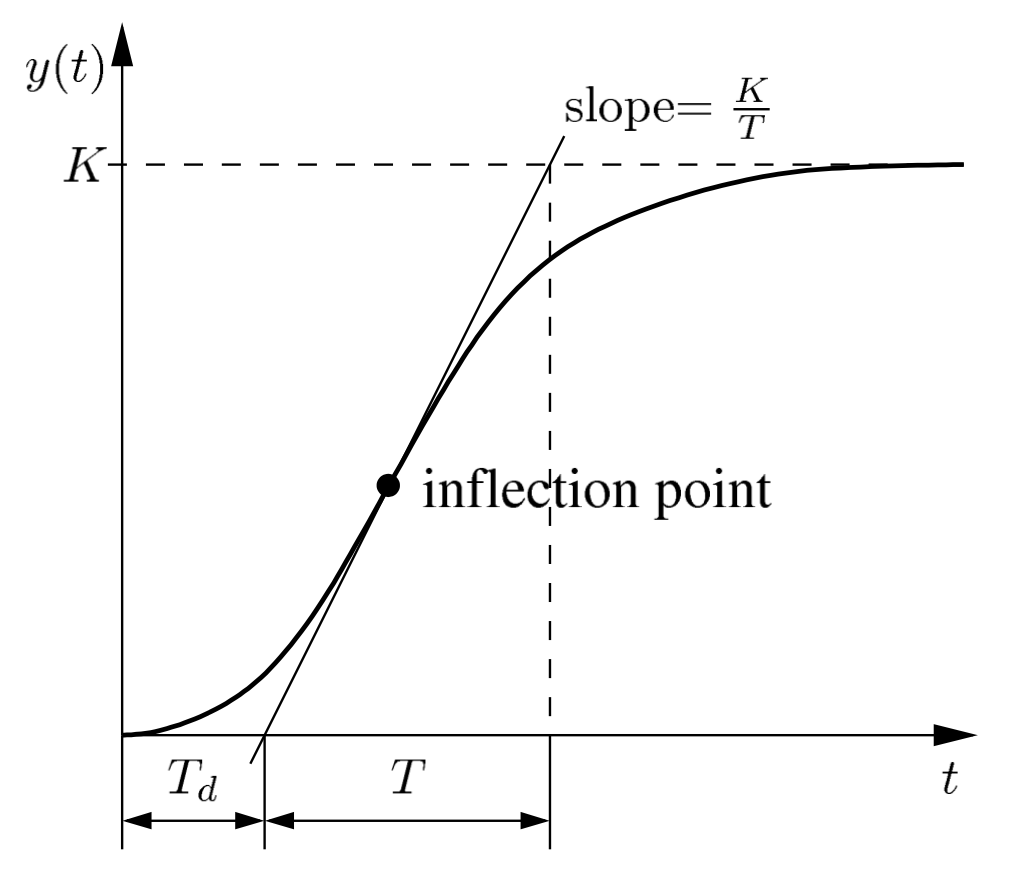
\includegraphics[width=1\linewidth]{fig/Dissli_Kienle_max_slope_2023.png}}
%
    \subcaptionbox{T-sum method \cite[Lecture 6, slide 17]{Dissli_Kienle_2023} \label{fig:condes:different_methods_Tsum}}[.45\textwidth]{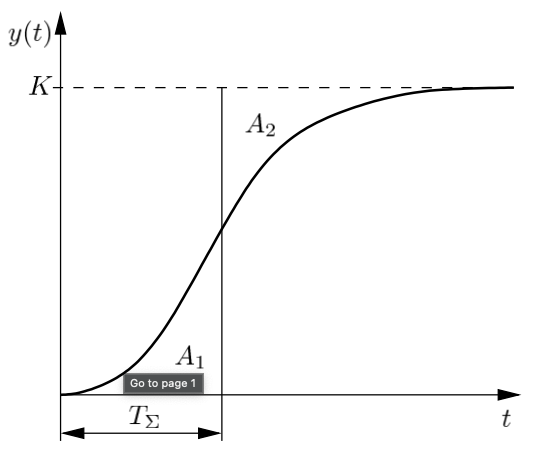
\includegraphics[width=1\linewidth]{fig/Dissli_Kienle_T_sum_2023.png}}
\\
\subcaptionbox{Two-point approximation \cite[Lecture 4, slide 6]{Dissli_Kienle_2023}  \label{fig:condes:different_methods_2p}}[.7\textwidth]{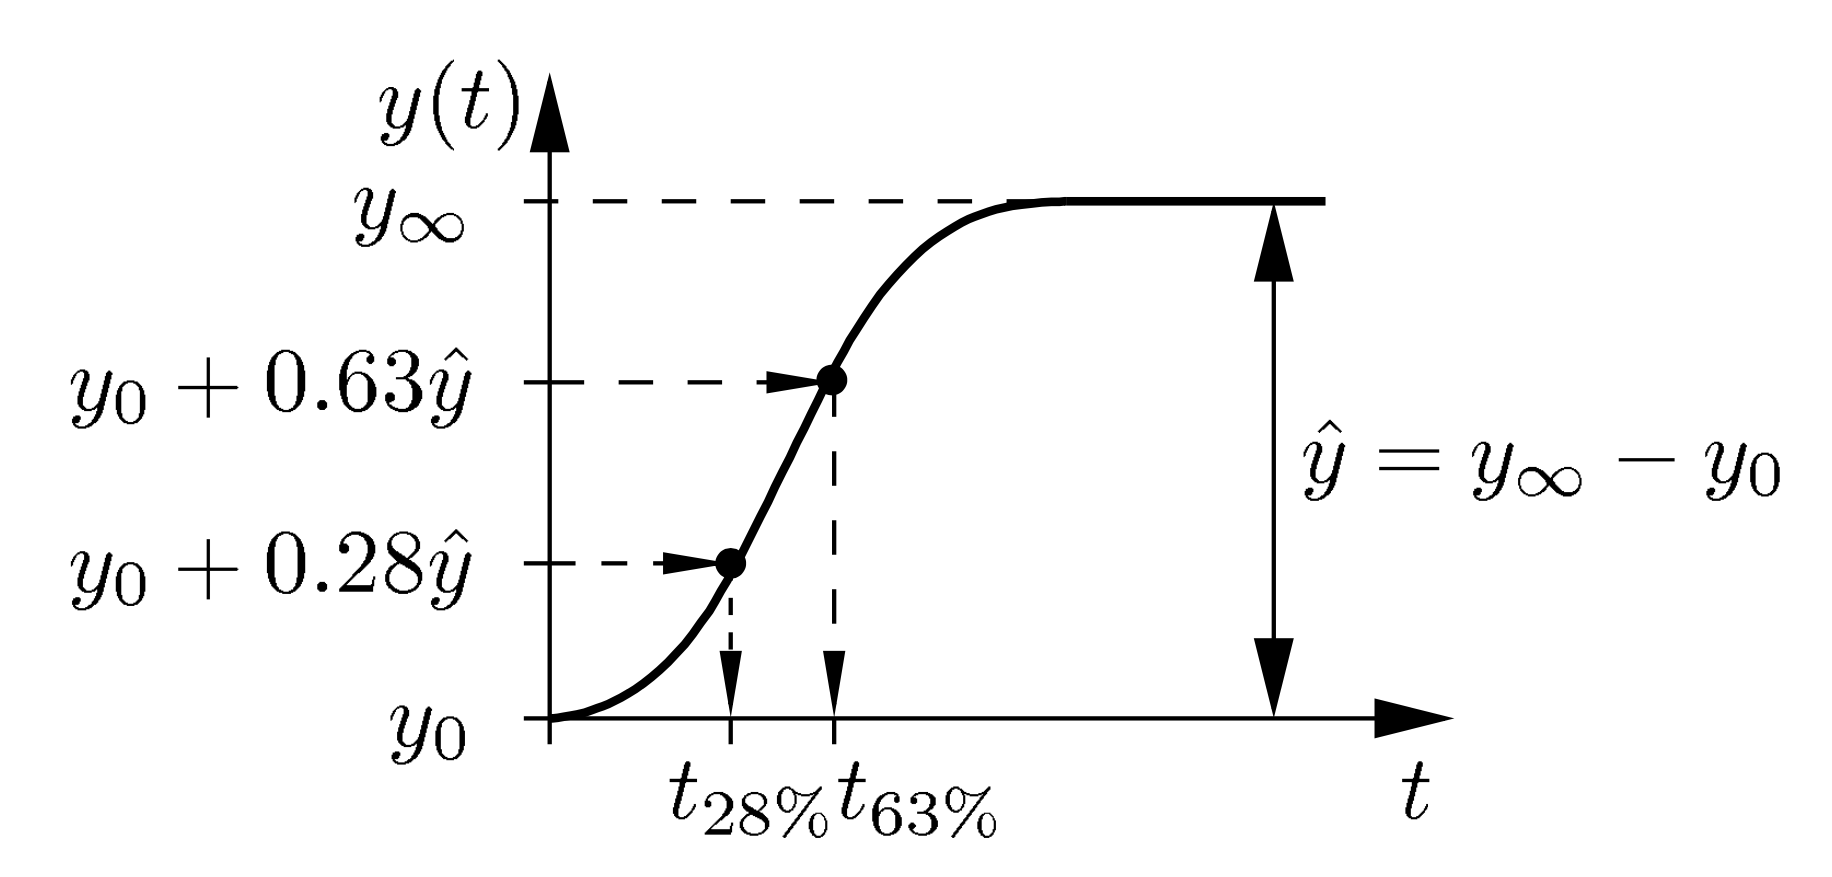
\includegraphics[width=1\linewidth]{fig/Dissli_Kienle_two_point_2023.png}}
    \caption{Visualization of two different approximation methods for Ziegler-Nichols controller design and the T-sum method for control parameter estimation. All plots from \cite{Dissli_Kienle_2023}}
    \label{fig:condes:different_methods}
\end{figure}


%Third, the relay-feedback method (\autoref{sec:condes:Relayfeedback}) as an example of an auto-tuning methods characterizes the control parameters.

In the end all methods are discussed and the robustness of some methods is shown (\autoref{sec:condes:discussion}).



\subsection{Ziegler-Nichols open loop method}\label{sec:condes:ZN}

The Ziegler-Nichols open loop method assumes an s-shape step response or an underlying first-order-plus-time-delay transfer function, respectively.
Looking at the given transfer function by Fragoso et~al. (\cite[Table 2]{Fragoso_et_al_2017}), we do not have this behaviour.
Therefore, we need to approximate a FOPTD transfer function.
This can be done with two different approaches.
First, the max-slope approximation is used for controller design and second, the two-point method determines the controller's parameters.

In the following two subsection both methods and their Matlab implementation is discussed. 


\subsubsection{Max-slope approximation} \label{sec:condes:ZN:maxS}

The max-slope method focuses around the inflection point of the unit step response.

\begin{lstlisting}[style=Matlab-editor,caption={This code snippet show the general way of calculating the control parameters with the max-slope method.},captionpos=b,label={list:condes:maxS}]
[y,t_out] = step(G,t_linspace);
[slope, intcpt] = calc_infliction_point_slope(y,t_out);
tngt = slope*t_out + intcpt;
[K, T, T_d, t_inter] = calc_gain_time_const_time_delay(y,t_out,tngt);
\end{lstlisting}

In line 1 the step response of a transfer function \texttt{G} with the Matlab built-in-function \texttt{step()} is calculated.
\texttt{calc\_infliction\_point\_slope()} calculates the infliction point and returns the slope (\texttt{slope}) and y-interception (\texttt{intcpt}) of the tangent at that point.
With these two values the tangent (\texttt{tngt}) is calculated in line 3 and in line 4 the variables needed for calculation of the control parameters are returned (\texttt{calc\_gain\_time\_const\_time\_delay()}).

The \texttt{calc\_infliction\_point\_slope()}-function calculates the gradient using Matlabs \texttt{gradient()}-function and computes slope and y-interception from this.

In \texttt{calc\_gain\_time\_const\_time\_delay()} the values for the maximal gain $K$, the time delay $T_d$, the time constant $T$ and the time of interception is computed and returned.

The complete functions can be found in the appendix (\autoref{app:ZN:infl_point}, \autoref{app:ZN:control_para}).

\subsubsection{Two-point approximation} \label{sec:condes:ZN:2p}

The aforementioned method uses the \texttt{gradient()}-function, which is sensitive to noise and outliers.
A more robust approach is the two-point method.
In \autoref{fig:condes:different_methods_2p} we see the points where 28\% and 63\% of $y_{\infty}$ is reached.
These values are calculated via Matlab and used to compute $T$, $T_d$ and $K$.
\begin{align}
    T &= \frac{2}{3} \left( t_{63} - t_{28} \right) \\
    T_d &= t_{63} - T \\
    K &= y_{\infty}
\end{align}

In matlab the computation relies on the \texttt{interp1()}-function.

\begin{lstlisting}[style=Matlab-editor,caption={This code snippet shows the general way of calculating $t_{28}$ and $t_{63}$.},captionpos=b,label={list:condes:maxS}]
[y,t] = step(G,t_linspace);
% Get maximum value of y
y_inf = max(y);
y_0 = min(y);
y_hat =  y_inf-y_0;
y_28 = y_0 + 0.28 * y_hat;
y_63 = y_0 + 0.63 * y_hat;
% Making y unique valued
[y_out,i_unique,~] = unique(y,'stable');
t_out = t(i_unique);
% Calculation of time points where y reaches 28/63 percent
t_28 = interp1(y_out,t_out,y_28);
t_63 = interp1(y_out,t_out,y_63);
\end{lstlisting}

First, $y_{28,63}$ is calculated and afterwards $t_{28,63}$ is computed by interpolation.
%Second, the corresponding $t$-values are calculated using the built-in \texttt{interp1()}-function for interpolation.
In line 9 the \texttt{unique()}-function returns all values of \texttt{y} without repetition.
This step is important for the later interpolation in line 12 f.


\subsubsection{Results} \label{sec:condes:ZN:results}

Before presenting the results an Matlab specific issue with PID controller implementation must be addressed.
The Simulink \texttt{PID}-block uses the another notation for the PID controller's parameter, therefore a conversion is needed. 
This conversion is shown in \autoref{list:condes:conersion_PID_para}.

\begin{lstlisting}[style=Matlab-editor,caption={Conversion of the parameters calculated by the previously mentioned algorithms and the values required for Simulink PID block in Matlab.},captionpos=b,label={list:condes:conersion_PID_para}]
function PID_ideal = matlab_PID_paremters(PID)
    % Conversion for Simulink PID-block
    PID_ideal.P = PID.K_p;
    PID_ideal.I =1/PID.T_I;
    PID_ideal.D = PID.T_D;
end
\end{lstlisting}


\begin{table}[H]
    \caption{Results of PID controller design using Ziegler-Nichols.}
    \centering
    \begin{tabular}{cccccc} \toprule
        Approximation & $v_{wind}$ [\si{\metre\per\second}] &$P$ & $I$ & $D$ & Input-Output pair \\ \midrule
        max-slope     & 7 & -1.0567 & 6.0606  & 1.5152 & 1-1 \\
        two-point     & 7 & -0.4121 & 10.1010 & 2.5253 & 1-1 \\
        max-slope     & 8 & -1.0781 & 8.0808  & 2.0202 & 1-1 \\
        two-point     & 8 & -0.4554 & 12.1212 & 3.0303 & 1-1 \\
        max-slope     & 9 & -0.1923 & 8.0808  & 2.0202 & 1-1 \\
        two-point     & 9 & -0.0844 & 12.1212 & 3.0303 & 1-1 \\ \bottomrule
    \end{tabular}
    \label{tab:condes:ZN:results}
\end{table}

\begin{figure}[H]
    \centering

    \subcaptionbox{Max-slope \label{fig:condes:ZN:results:max_slope_example}}[.48\textwidth]{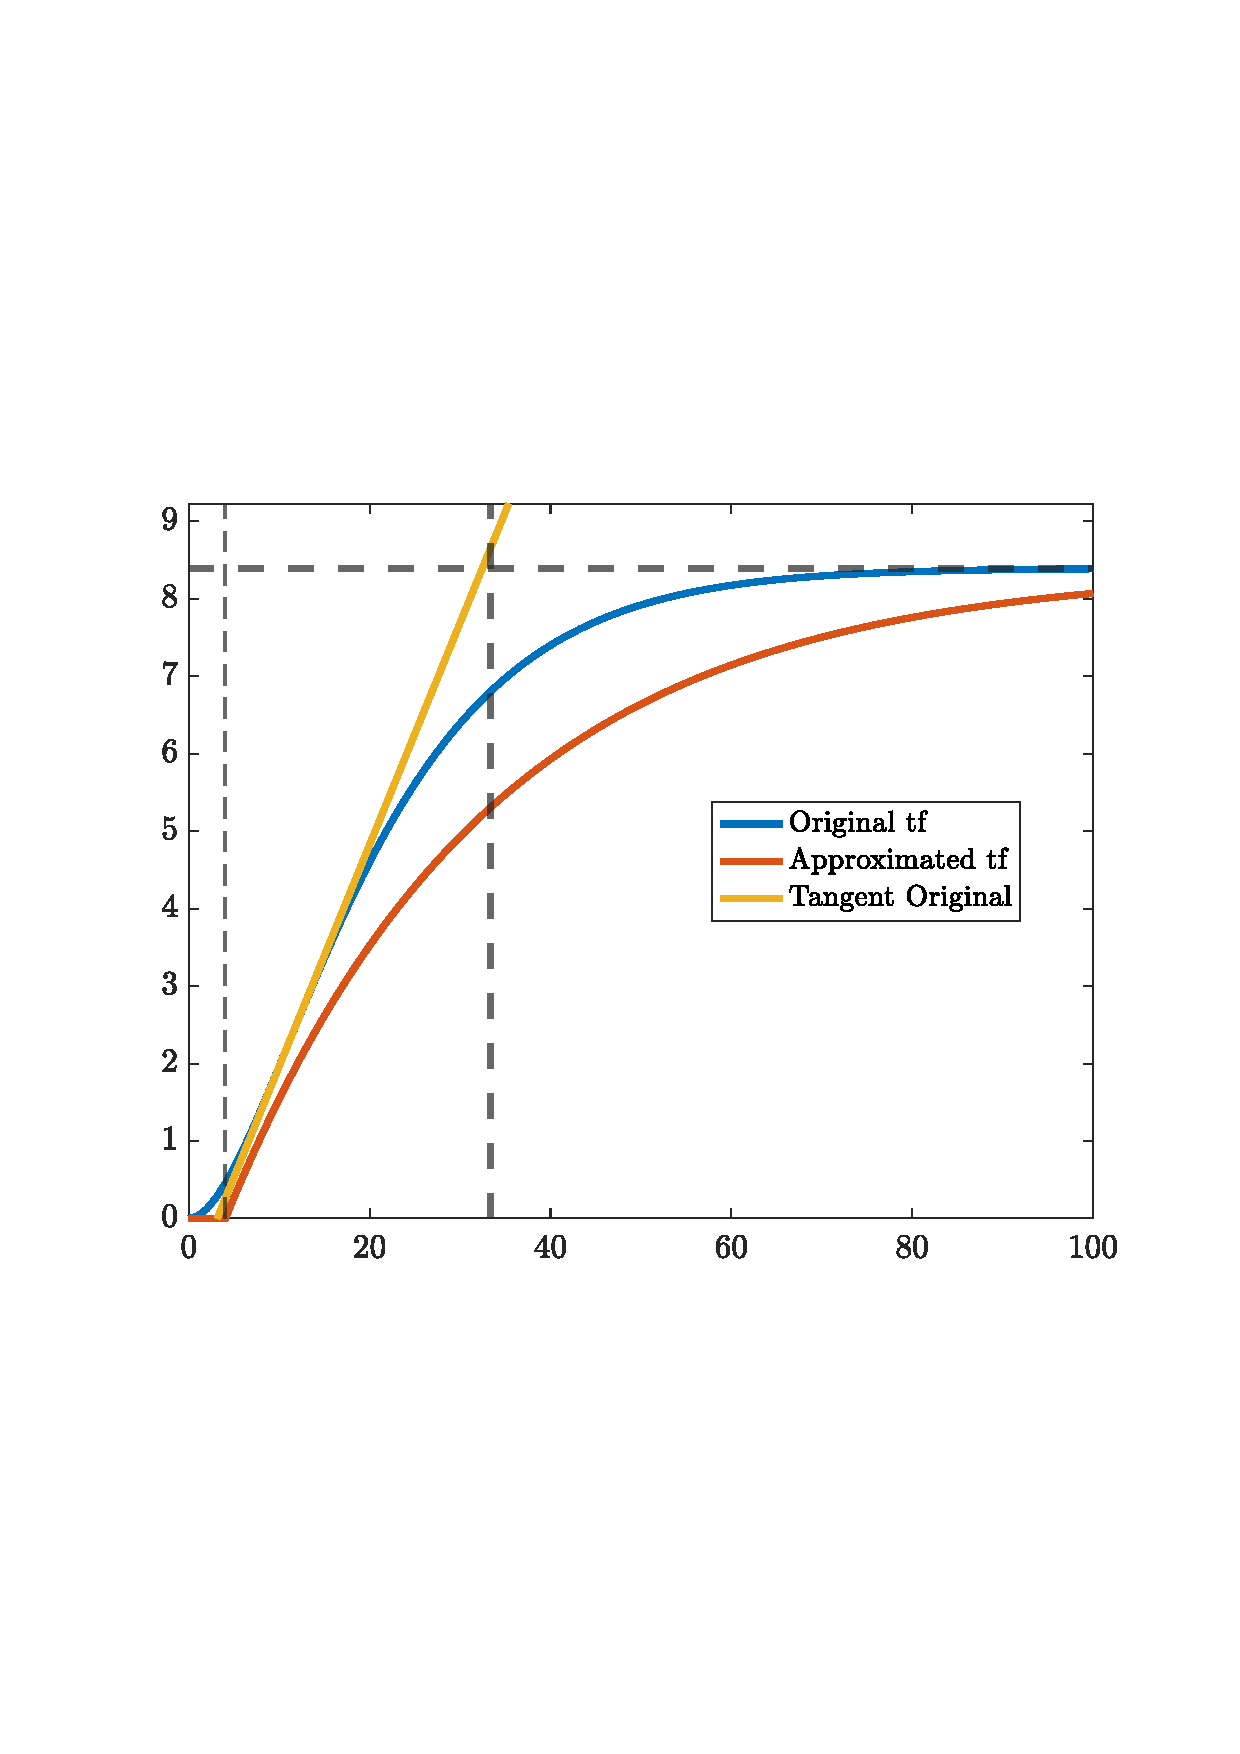
\includegraphics[width=1\linewidth, scale=1, trim=75 230 55 120,clip]{fig/G_11_max_slope_8ms.pdf}}
%
    \subcaptionbox{Two-point \label{fig:condes:ZN:results:2p_example}}[.48\textwidth]{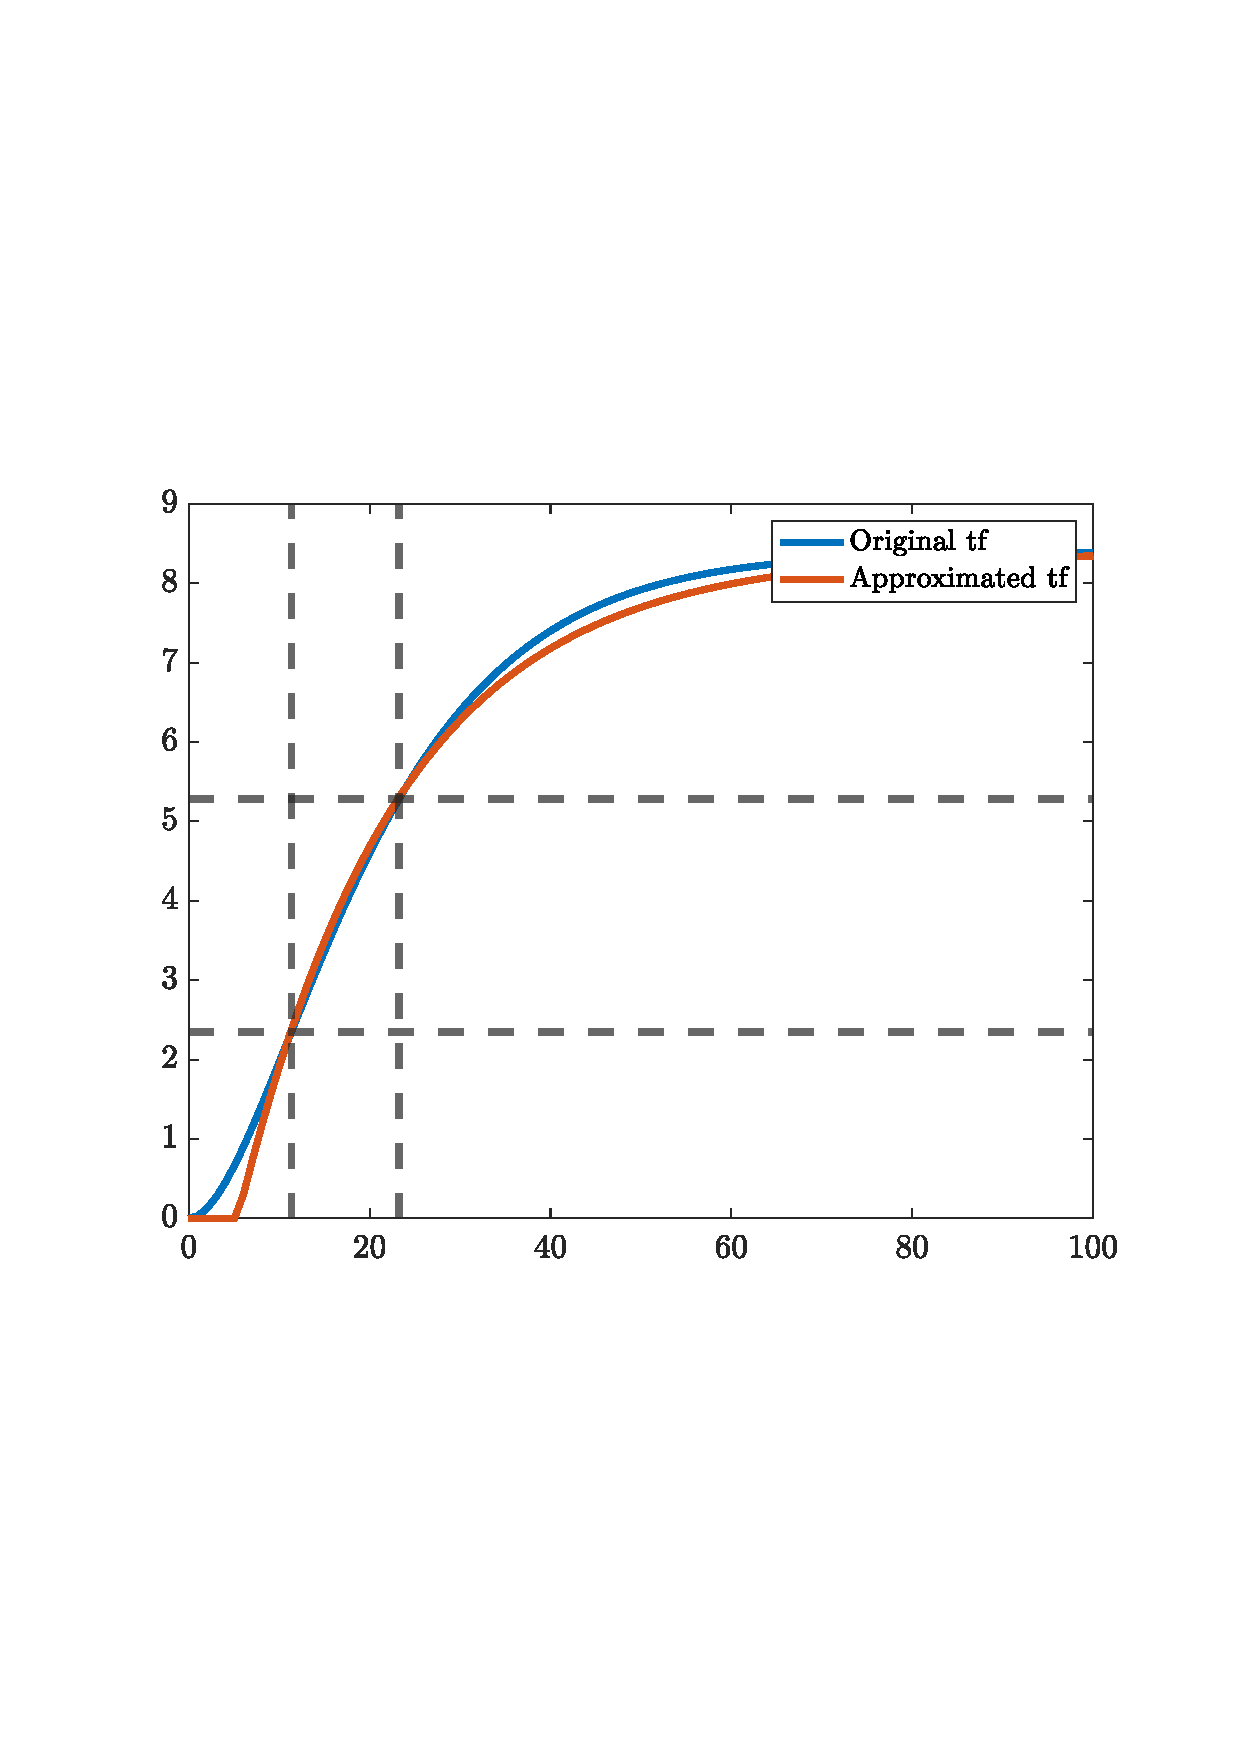
\includegraphics[width=1\linewidth, scale=1, trim=75 230 55 120,clip]{fig/G_11_2p_8ms.pdf}}

    \caption{Approximation of the transfer function at a wind speed of \SI{8}{\metre\per\second} and using the input-output pair 1-1}
    \label{fig:condes:ZN:results:example_plots}
\end{figure}

In \autoref{fig:condes:ZN:results:example_plots} we can clearly see the difference of approximation comparing max-slope and two-point method.
The result of the difference in approximation are different control parameter (\autoref{tab:condes:ZN:results}).
Still, the sign of all control parameters are equal and the differences are small.
When the wind speed is changed (using a different transfer function) the proportional factor $P$ of the PID controller changes.
The integral $I$ and derivative $D$ terms seem be constant.

\subsection{T-sum method} \label{sec:condes:Tsum}

For the input-output pair 2-2 we use the T-sum method.
T-Sum tries to find a line where two integrals have the same area. 
One is the area enclosed by the y-axis and the solution trajectory.
The other area is border by the solution trajectory and the $y_{\infty}$-value.
By shifting the dashed line seen in \autoref{fig:condes:tsum:example} on the $y$-axis the optimal point of equal areas is found.
The controller's parameters are calculated by $T_{\Sigma}$.
\begin{align}
    P &= \frac{1}{K} \\
    I &= 0.667 \cdot T_{\Sigma} \\
    D &= 0.167 \cdot T_{\Sigma}
\end{align}

\begin{table}[H]
    \caption{Results of PID controller design using T-Sum method.}
    \centering
    \begin{tabular}{ccccc} \toprule
        $v_{wind}$ [\si{\metre\per\second}] &$P$ & $I$ & $D$ & Input-Output pair \\ \midrule
        7 & 0.1724 & 0.6737 & 0.1687 & 2-2 \\
        8 & 0.1479 & 0.6737 & 0.1687 & 2-2 \\ 
        9 & 0.1240 & 0.6737 & 0.1687 & 2-2 \\ \bottomrule
    \end{tabular}
    \label{tab:condes:tsum:results}
\end{table}

\begin{figure}[H]
    \center
    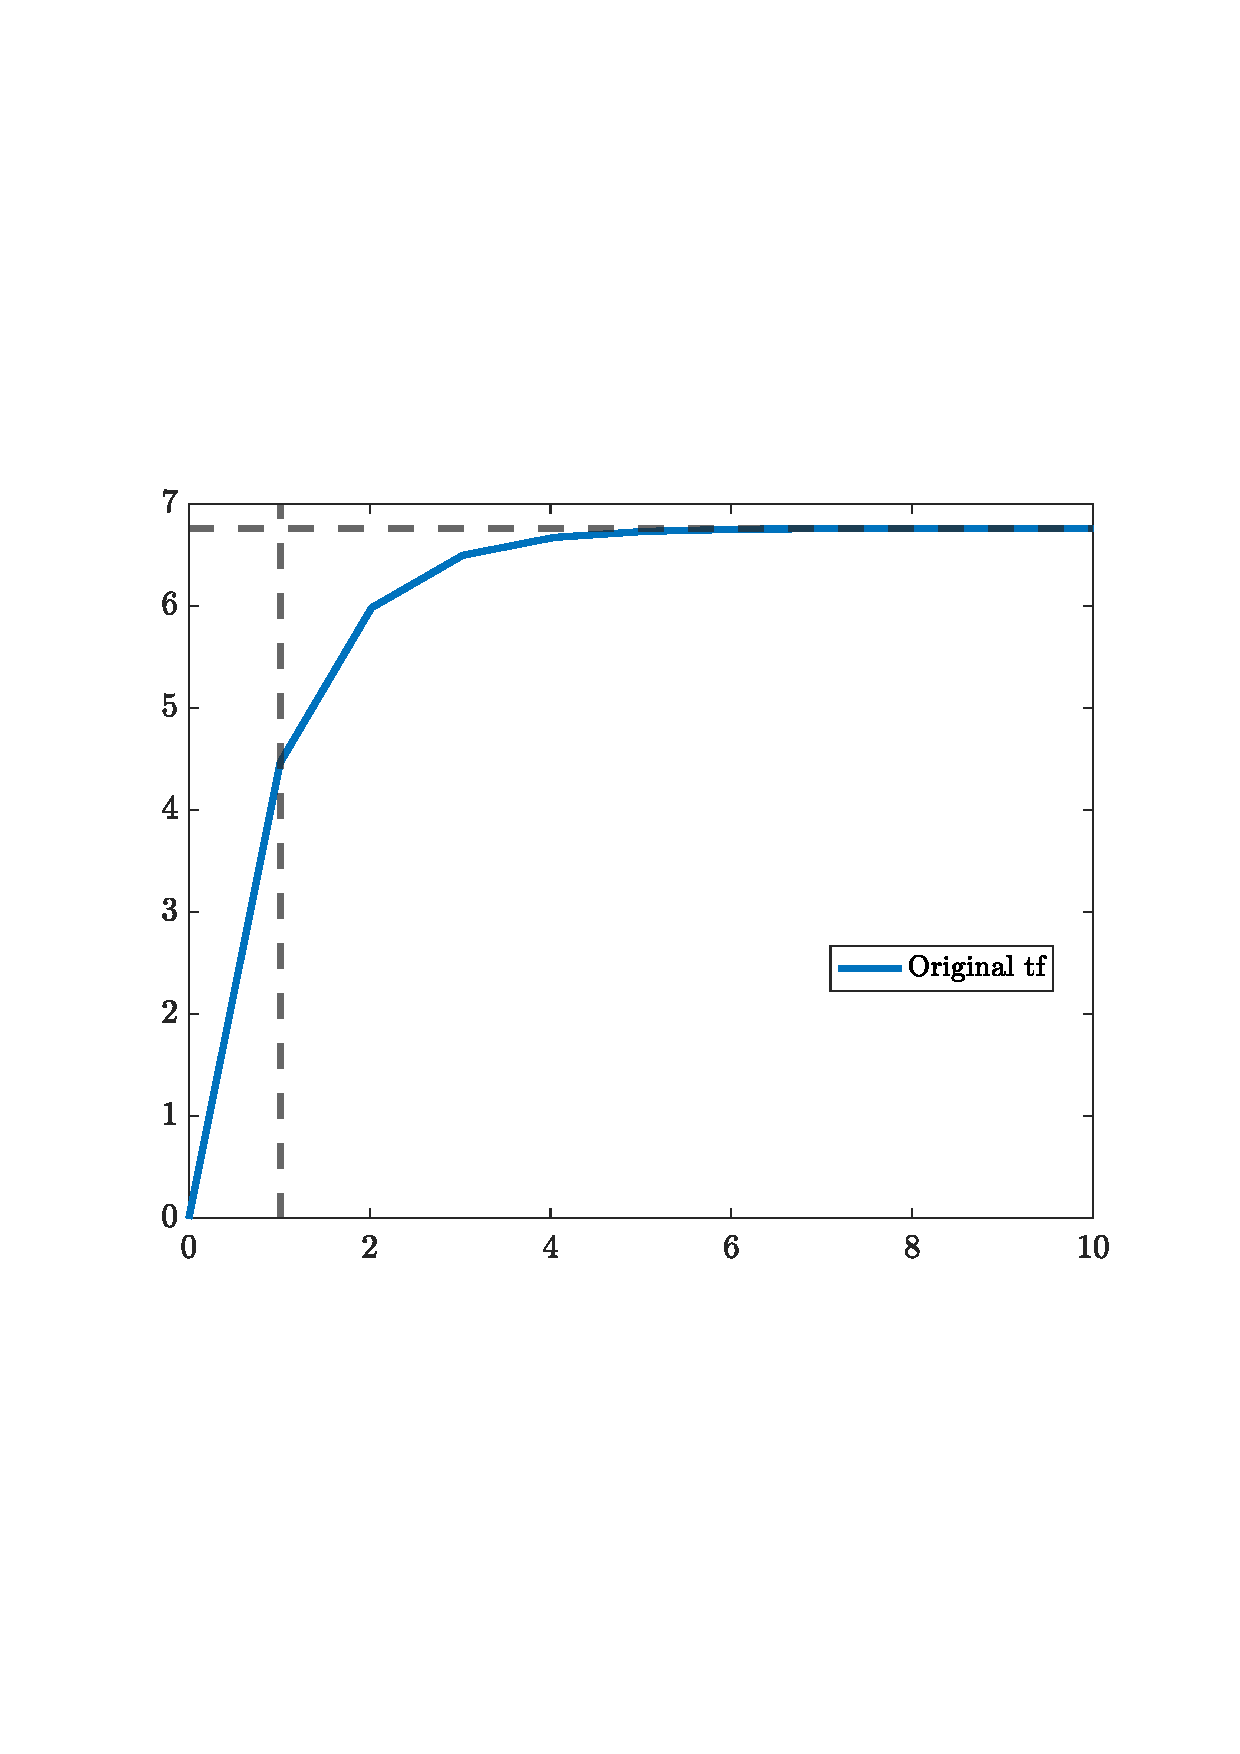
\includegraphics[scale=0.7,trim=60 200 50 150,clip]{fig/G_22_T_sum_8ms.pdf}
    \caption{Visualization of the T-sum method for controller design. A controller for the input-output pair 2-2 is designed by using the transfer function for a windspeed of \SI{8}{\metre\per\second}.}
    \label{fig:condes:tsum:example}
\end{figure}

%\autoref{fig:condes:tsum:example} shows one possible downside of the T-sum method. 
%When simulating the system the resulting solution is a discrete vector.

%\subsection{Relay-feedback method} \label{sec:condes:Relayfeedback}

\subsection{Implementation in Simulink} \label{sec:condes:implementation_simulink}

In the previous subsection the design of the controller is discussed.
Now, the implementation of the closed and open loop is addressed.
In contrast to the controller design, the closed and open loop is implemented in Simulink.

\subsubsection*{Open loop} \label{sec:condes:implementation_simulink:open_loop}

In general two different approaches for the implementation are possible.
The transfer function can be arranged as a structured flow diagram (\autoref{fig:condes:implementation:structure}).
In this case each transfer function is implemented individually in a single Simulink \texttt{tf-block}.
One advantage is that the overall structure of the system is visible and all \textit{flows of informations} are visible.
Otherwise, this implementation is more complex and therefore more error-prone.

The second case is a more condensed implementation (\autoref{fig:condes:implementation:block}).
In this, only two Simulink \texttt{LTI}-blocks are used for the system $G$ and the disturbance $G_D$.

\begin{figure}[H]
    \centering

    \subcaptionbox{Implementation as a structure \label{fig:condes:implementation:structure}}[.48\textwidth]{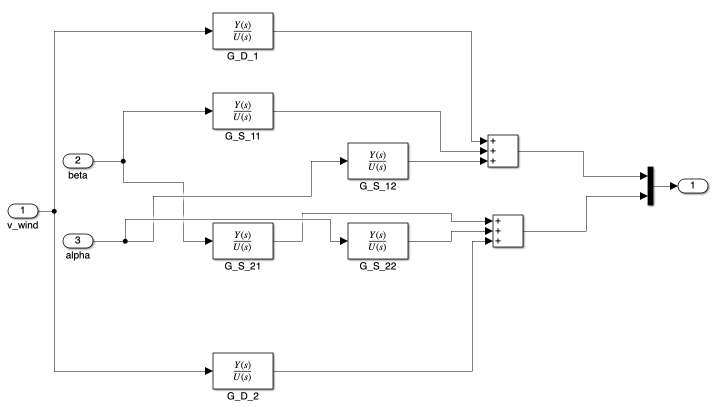
\includegraphics[width=1\linewidth, scale=1, trim=0 0 0 0,clip]{fig/Simulink/simulink_tf_structure.png}}
%
    \subcaptionbox{Implementation as blocks  \label{fig:condes:implementation:block}}[.48\textwidth]{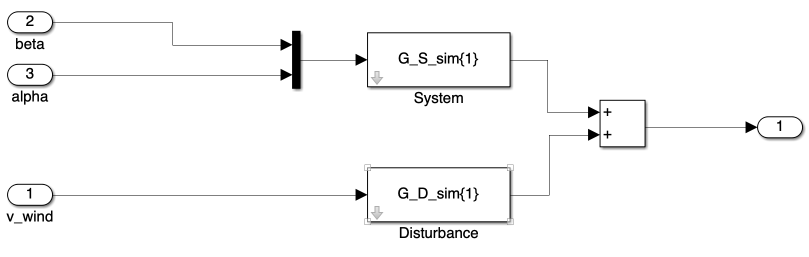
\includegraphics[width=1\linewidth, scale=1, trim=0 0 0 0,clip]{fig/Simulink/simulink_tf_block.png}}

    \caption{Comparing the two different approaches as Simulink block diagrams. The \textit{structured} implementation (\texttt{transfer\_function\_structured.slx}) reveals much more details about the internal dependencies. A more condensed view is seen for the \textit{block} implementation (\texttt{transfer\_function\_as\_block.slx}).}
    \label{fig:condes:implementation:two_approaches}
\end{figure}

To check the implementation it is good to use both implementation in parallel and check if both are getting the same results.
For further investigation the \textit{structured} implementation can be used.
This has the advantage that \textit{internal flows} or states can be monitored with Simulinks \texttt{scope}- or \texttt{out}-blocks.

\begin{figure}[H]
    \center
    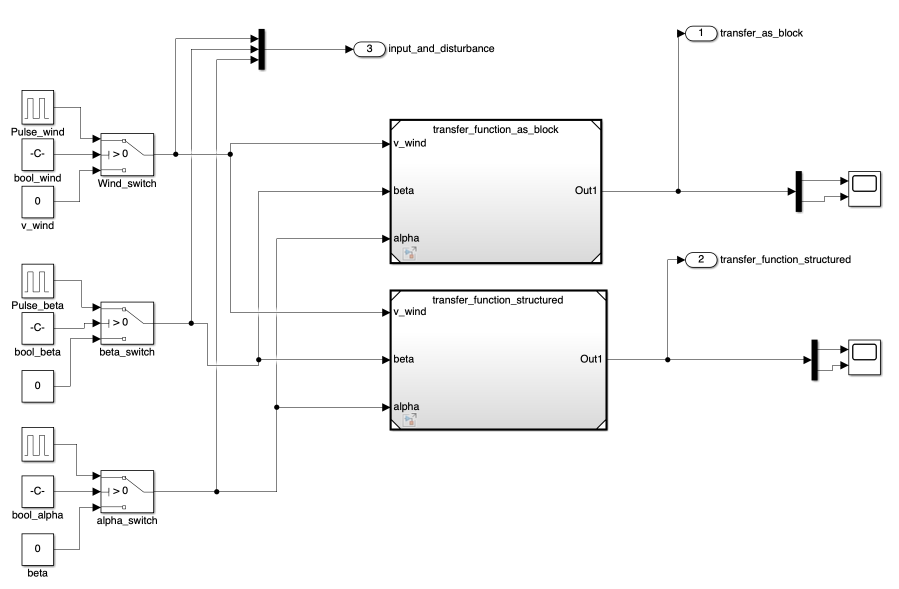
\includegraphics[width=1\textwidth,scale=1,trim=0 0 0 0,clip]{fig/Simulink/simulink_open_loop.png}
    \caption{The open loop system with a parallel execution of \textit{structured} and \textit{block} implementation. This figure is showing the \texttt{step\_response\_open\_loop.slx}-file.}
    \label{fig:condes:implementation:openloop}
\end{figure}

The Simulink file shown in \autoref{fig:condes:implementation:openloop} has three outputs.
\texttt{out1} returns the open loop behaviour for the \texttt{block} implementation, the second output (\texttt{out2}) for the \texttt{structured} implementation. 
The third \texttt{output}-block is to check the inputs into the system.

For each of the three inputs $v_{wind}$ (disturbance), $\beta$ and $\alpha$ (from top to down) a \texttt{switch}-block is used (see left side of the Simulink diagram).
These \texttt{switch}-blocks allow to choose via a flag set in a Matlab script which input should have a pulse applied to.
The pulse is produced by an \texttt{pulse}-block in Simulink.

\autoref{list:condes:implementation:flags} shows how to choose different scenarios depending on flags and \texttt{switch}-blocks.
Lines 7 ff. determine which pulse is given to system.
If the variable is set to $0$ the input does not have a pulse signal applied to, and it is constant $0$.
In the given example only $\beta$ will receive a pulse of magnitude \SI{7}{\degree} and a width of \SI{600}{\second} after \SI{600}{\second} of simulation time.

\begin{lstlisting}[style=Matlab-editor,caption={Setting flags for different combination of input pulses.},captionpos=b,label={list:condes:implementation:flags}]
% Setting amplitudes for pulse
simP.A_beta = 7;
simP.A_alpha = -.1;
simP.A_wind = -2;

% Determine if pulse of zero for inputs and disturbance
simP.bool_beta = 1;
simP.bool_alpha = 0;
simP.bool_wind = 0;

% Simulation paramters
simP.t_simulation = 2000; % Time for simulation [s]
simP.T_period = 1200;     % Peroid of pulse [s]
simP.T_delay = 600;       % Delay for first pulse [s]
simP.pulse_width = 50;    % Pulse width in % of T_Period [%]
\end{lstlisting}


\subsubsection*{Closed loop} \label{sec:condes:implementation_simulink:closed_loop}

When the designed controllers are tested the loop must be closed.

\begin{figure}[H]
    \center
    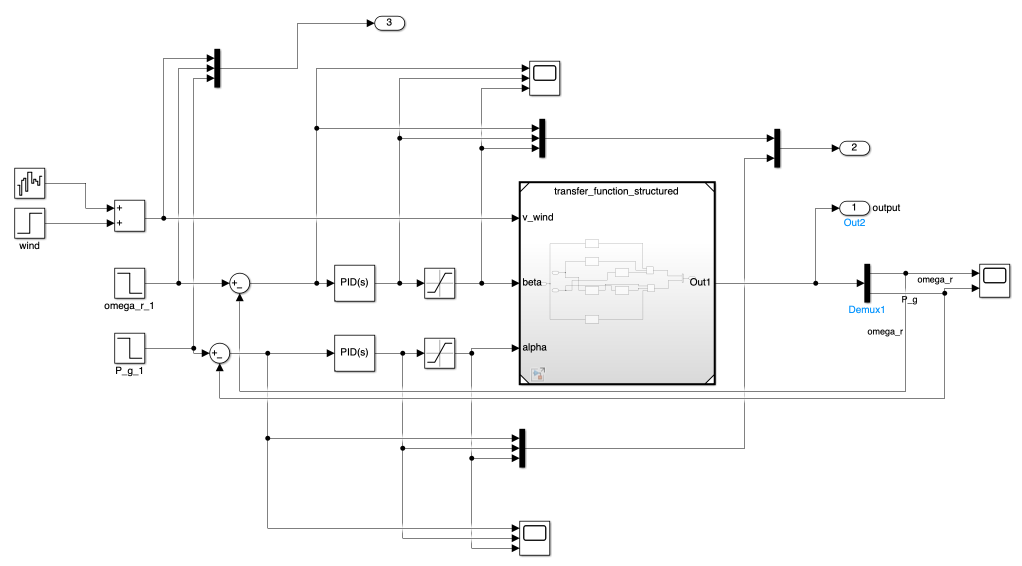
\includegraphics[width=1\textwidth,scale=1,trim=0 0 0 0,clip]{fig/Simulink/simulink_closed_loop.png}
    \caption{The closed loop with a \texttt{PID}-controller block, both reference signals and a possible disturbance due to wind. This figure is showing the \texttt{closed\_loop\_PID.slx}-file.}
    \label{fig:condes:implementation:closedloop}
\end{figure}

For possible disturbance due to a change in wind speed a \texttt{step}- and a \texttt{noise}-block is added.
With this setup, not only can the wind change drastically (step change, boe) but also naturally occurring fluctuation can be simulated.
After the \texttt{PID}-block a \texttt{saturation}-block is added.
\autoref{sec:condes:discussion} discusses the need of having a saturation block, which enforces the limitations of input signals shown in \autoref{tab:analysis:constraints}.
